Two students stretch a long slinky. Each sends a pulse towards the other at \vO: one up, one down, of the same shape. The diagram shows the spring at $t = 0$.

\begin{center}
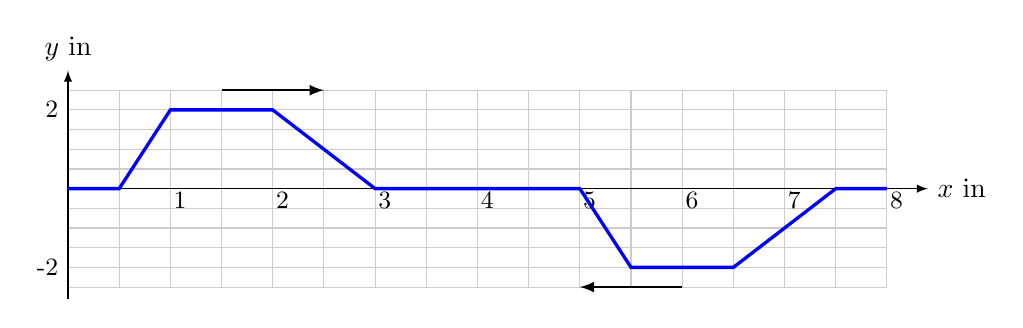
\begin{tikzpicture}[>=latex, x=1.3cm, y=0.5cm]
 \draw[gray!40, step=0.5] (0,-2.5) grid (8,2.5);
 \draw[->] (0,0) -- (8.4,0) node[right] {$x$ in \si{\m}};
 \draw[->] (0,-2.8) -- (0,3) node[above] {$y$ in \si{\cm}};
 \foreach \x in {1,...,8} \node[below right, inner sep=1pt] at (\x,0) {\small \x};
 \foreach \y in {-2,2} \node[left] at (0,\y) {\small \y};
 \draw[very thick, blue] (0,0) -- (0.5,0) -- (1,2) -- (2,2) -- (3,0) -- (5,0) -- (5.5,-2) -- (6.5,-2) -- (7.5,0) -- (8,0);
 \draw[->, thick] (1.5,2.5) -- (2.5,2.5);
 \draw[->, thick] (6,-2.5) -- (5,-2.5);
\end{tikzpicture}
\end{center}

\begin{abcliste}
\abc When is the spring straight for a moment?

\abc Where is the energy of the pulses at that moment?
\end{abcliste}
